\documentclass[12pt,a4paper]{article}
%\usepackage[utf8]{inputenc}
%\usepackage[T1]{fontenc}
\usepackage{xeCJK}
\usepackage{setspace} 
\usepackage{graphicx}

%
\setCJKmainfont{IPAMincho}
\setCJKsansfont{IPAGothic}
\setCJKmonofont{IPAGothic}


\title{私の家族のすきなレストラン\\\small{A Favorite Restaurant}}
\author{アンドリュー・ローゼン\\ \small{Andrew Rosen}\\\small{JPNS 1001-003}}
\date{}
\begin{document}
	\maketitle
	
	
	
	%\doublespacing
	
	私の家族のすきなレストランは。
	夏に東京に教えました。
	目黒駅の東口を出て、道を綿まて、右へ五分ぐらいです。
	トラットリア・イタリア目黒店は道の左側にあります。
	このレストランはうちの近くです。% TODO:  required
	\begin{figure}
		\centering
		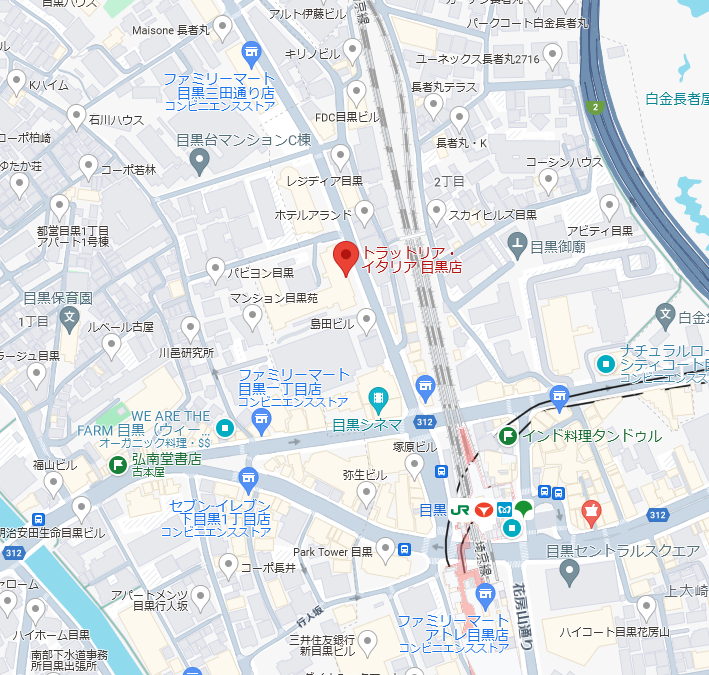
\includegraphics[width=0.7\linewidth]{restaurant}
		\caption{トラットリア・イタリア目黒店}
		\label{fig:restaurant}
	\end{figure}
	

\end{document}